\documentclass{article}
\usepackage[utf8]{inputenc}
\usepackage{graphicx}
\begin{document}


\begin{figure}
\centering    
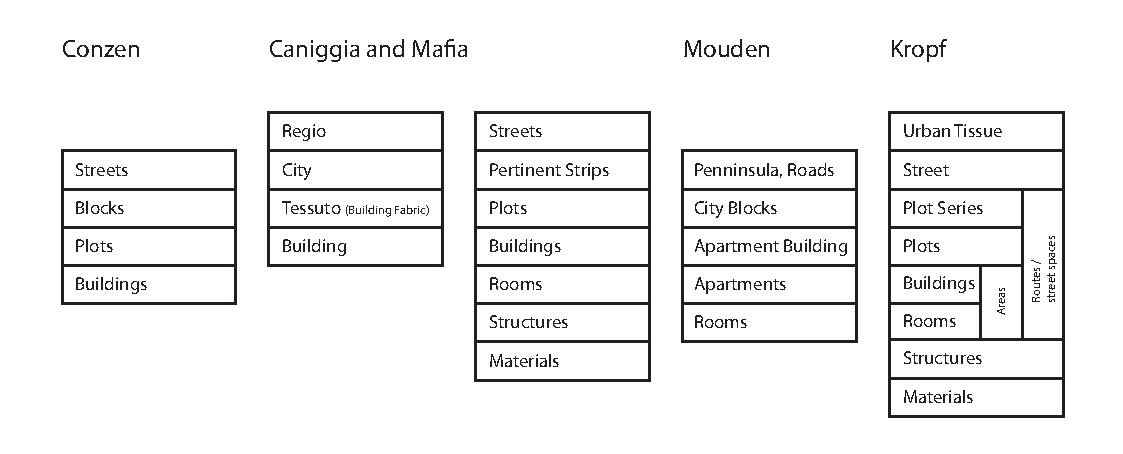
\includegraphics[scale=0.80,page=1]{Images/Typology_Dichtomies.pdf}  
\caption{\bf Different scales of dichotomies. }    
 \label{fig:TypologyDichtomies}  
\end{figure} 

\begin{figure}
    \centering    
\includegraphics[scale=0.5]{Images/Paris-StreetView-SampleLocations_crop.png}  
\caption{\bf Sampling locations for map imagery (from Paris, France) \cite{GoogleStatic2017}.}    
 \label{fig:parissample}  
\end{figure} 


\begin{figure}
    \centering  
 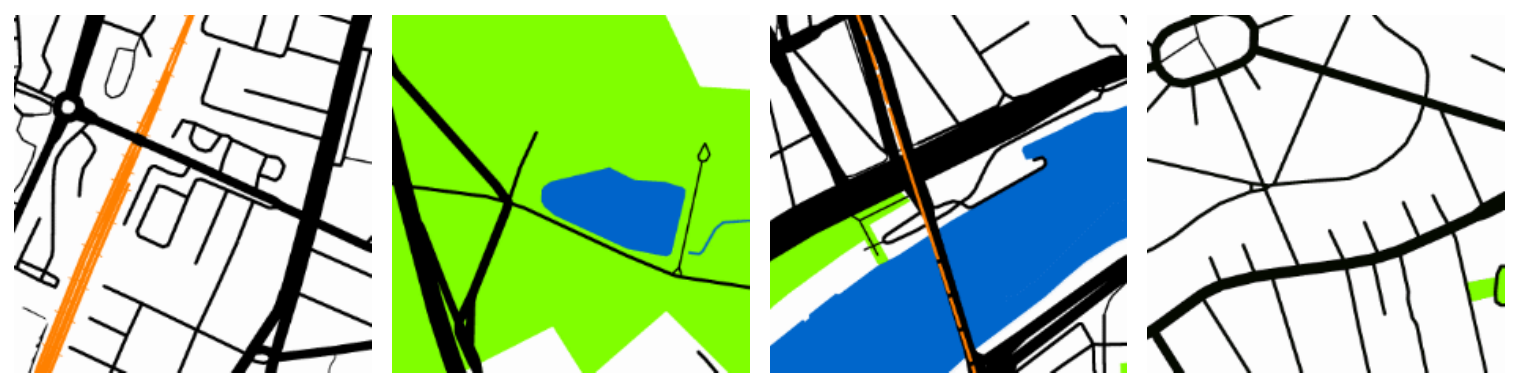
\includegraphics[scale=0.8]{Images/SampleTraining.png}     
\caption{\bf Four sample Google Maps training data images (from Paris, France) \cite{GoogleStatic2017}.}    
 \label{fig:maps}  
\end{figure} 

\begin{figure}
    \centering    
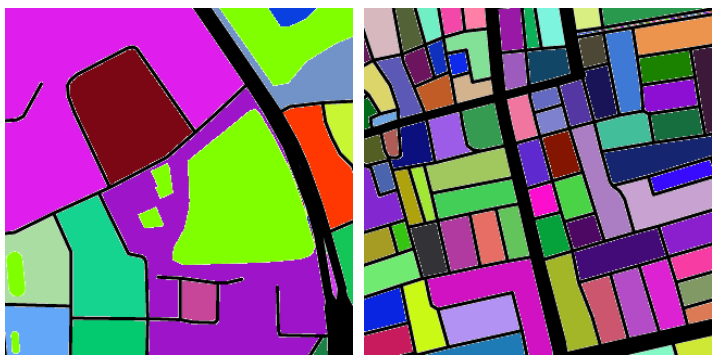
\includegraphics[scale=0.8]{Images/FloodSample.png}     
\caption{\bf Results of flood filled city blocks.}    
 \label{fig:floodfilled}  
\end{figure} 



\begin{figure}
    \centering    
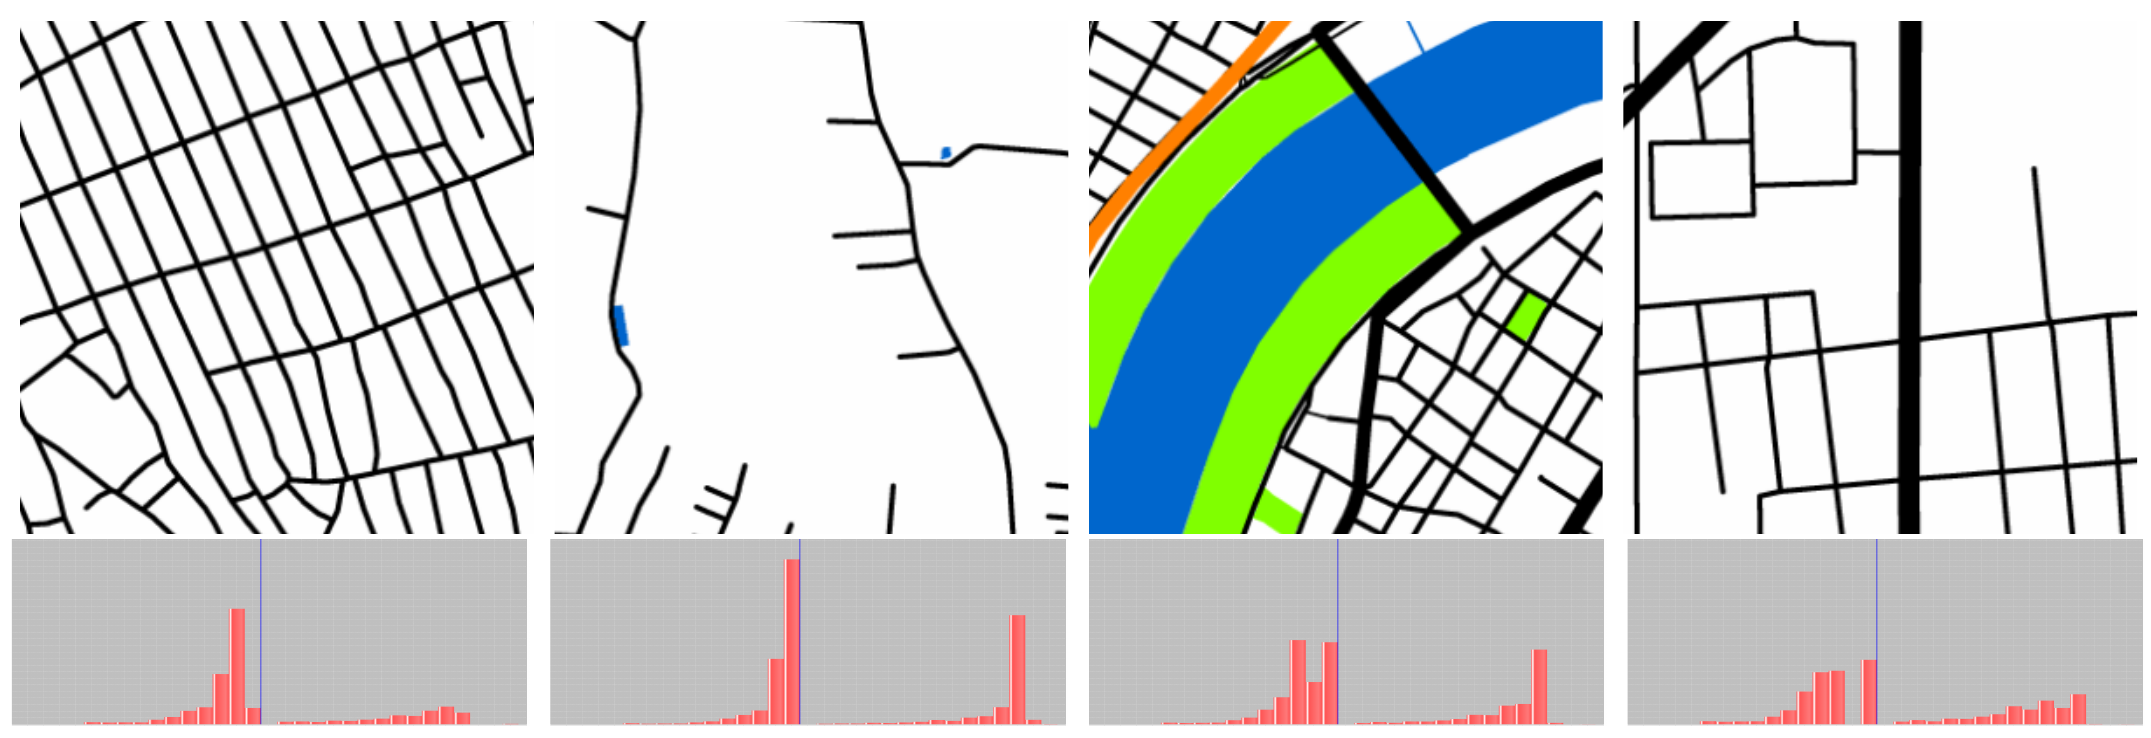
\includegraphics[scale=0.55]{Images/HistSamples.png}  
\caption{\bf Four samples of map regions (top) and resulting histograms (bottom). Region size and regularity are joined into a combined histogram, with size frequencies on the left side of the graph and regularity on the right.}    
 \label{fig:mapsandHist}  
\end{figure} 

\begin{figure}
\centering    
\includegraphics[scale=0.10]{Images/SomImages.png}  
\caption{\bf  A visualisation of the 2 dimensional SOM trained with 1.7 million map images.  Each x,y point shows Left: a representative image associated with each node while nodes without associated images are shown in black and Right: number of images associated with each node}    
 \label{fig:somresults}  
\end{figure} 

\begin{figure}
\centering    
\includegraphics[scale=0.70,page=1]{Images/Melbourne_5_Final.pdf}  
\caption{\bf  Map of Melbourne, Australia with 24027 individual map segments classified and colour coded. Note, the CBD shows additional points due to inclusion of the 1000 circular sampling procedure in addition to the 23,027 locations sampled at 400m resolution. }    
 \label{fig:mel23000}  
\end{figure} 




\end{document}